\chapter{Recommendations}
\section{Entrances}
\subsection{Introduction}\label{intro}
% this is a comment
% normal text
This section will describe the work that is done to find out what, when and how frequent entrances of the Faculty of Architecture are used. This is an interesting and challenging use case at the same time. The Faculty of Architecture is a building having multiple entrances; five to be precise. Knowing what, when and how frequent these entrances are used, will give insight into the use of a building, the spatial context and the relation between these two.
\subsection{Methodology}\label{method}
In order to find what entrance someone uses to enter or exit a building, we will look in the part of a sequence in which the device is recorded by an AP in a building and subsequently recorded by an AP in another building. More specific, we will look at what (first or last) AP is used in a movement from one to another building. For this two different approaches can be distinguished. The first approach does not take in account the devices that might get recorded when passing by the building. In  the second approach we will make use of the pre-processed data which excluded the passing by events.
\subsection{Hypothesis}\label{hypo}
Our hypothesis is that finding clear answers to the question whether it is possible to identify what entrances are most frequently used, is going to be hard. Firstly, because the existing layout of APs is not designed for the purpose of tracking people. For this reason there is not always an AP located near an entrance. Secondly, because the logging frequency of the system is a little more than 5 minutes. Ideally the system records the connected device at the very first AP it connects with. The chance the device is recorded at the moment it is connected with the very first access point is small. However we still expect to see some results. Although the time interval in which the system logs the connected devices is relatively large, an AP located near an entrance would still pop up as one of the most frequently used AP as first connection (assuming people disseminate over the building after entering). 
\subsection{First approach: including passing by events}
The first approach makes use of the raw wifilog data, by finding the part in a sequence in which a device is recorded by an AP in a building and is subsequently recorded in another building. The states in which a device is scanned once are not filter out. These single records imply that a device only passed by the building, and thus was not located in the building. \\\\
\begin{figure}[H]
	\centering
	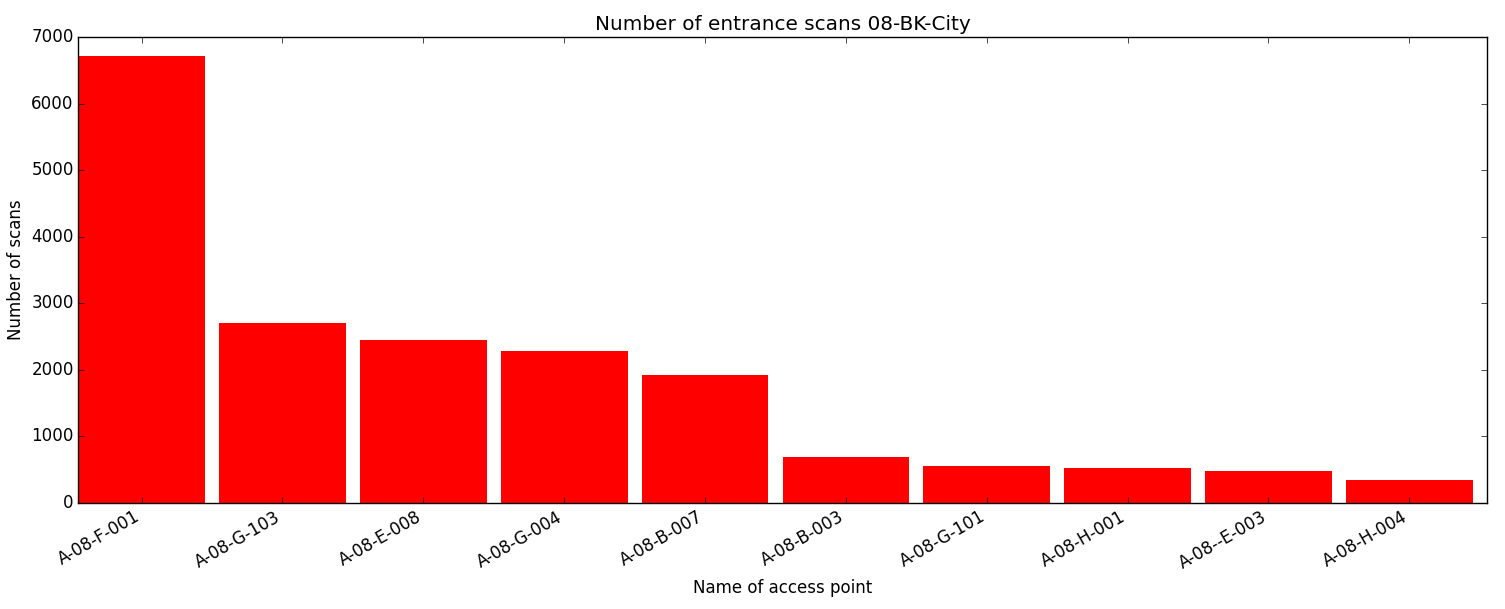
\includegraphics[scale=0.2]{entrances_firstapproach_1.png}
	\captionsetup{justification=centering}
	\caption{Most frequently recorded APs in a movement to the Faculty of Architecture}
	\label{firstapproach_graph}
\end{figure}
\begin{figure}[H]
	\centering
	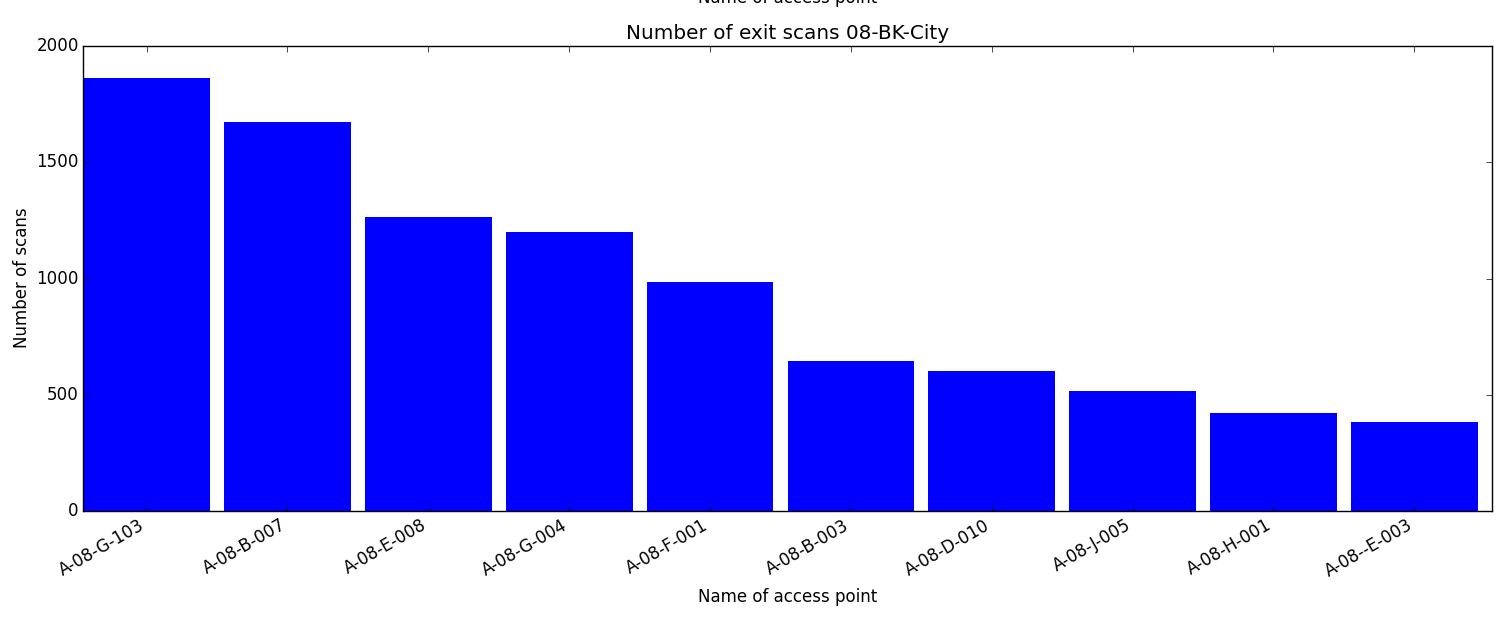
\includegraphics[scale=0.2]{entrances_firstapproach_2.png}
	\captionsetup{justification=centering}
	\caption{Most frequently recorded APs in a movement from the Faculty of Architecture}
	\label{firstapproach_graph}
\end{figure}
The floor plans of the Faculty of Architecture, enriched with the location of APs, are used to locate the most frequently used APs on the map (see ??). The result is interesting, since most APs are not located near an entrance but are located at one of the corners of the building. Most of the them are located at the western part of the building. Knowing that lots of people are passing in the street next to this part of the building, we can conclude the result of this analysis is distorted due not filtering out the devices that are recorded when passing by the building.
\begin{figure}[H]
	\centering
	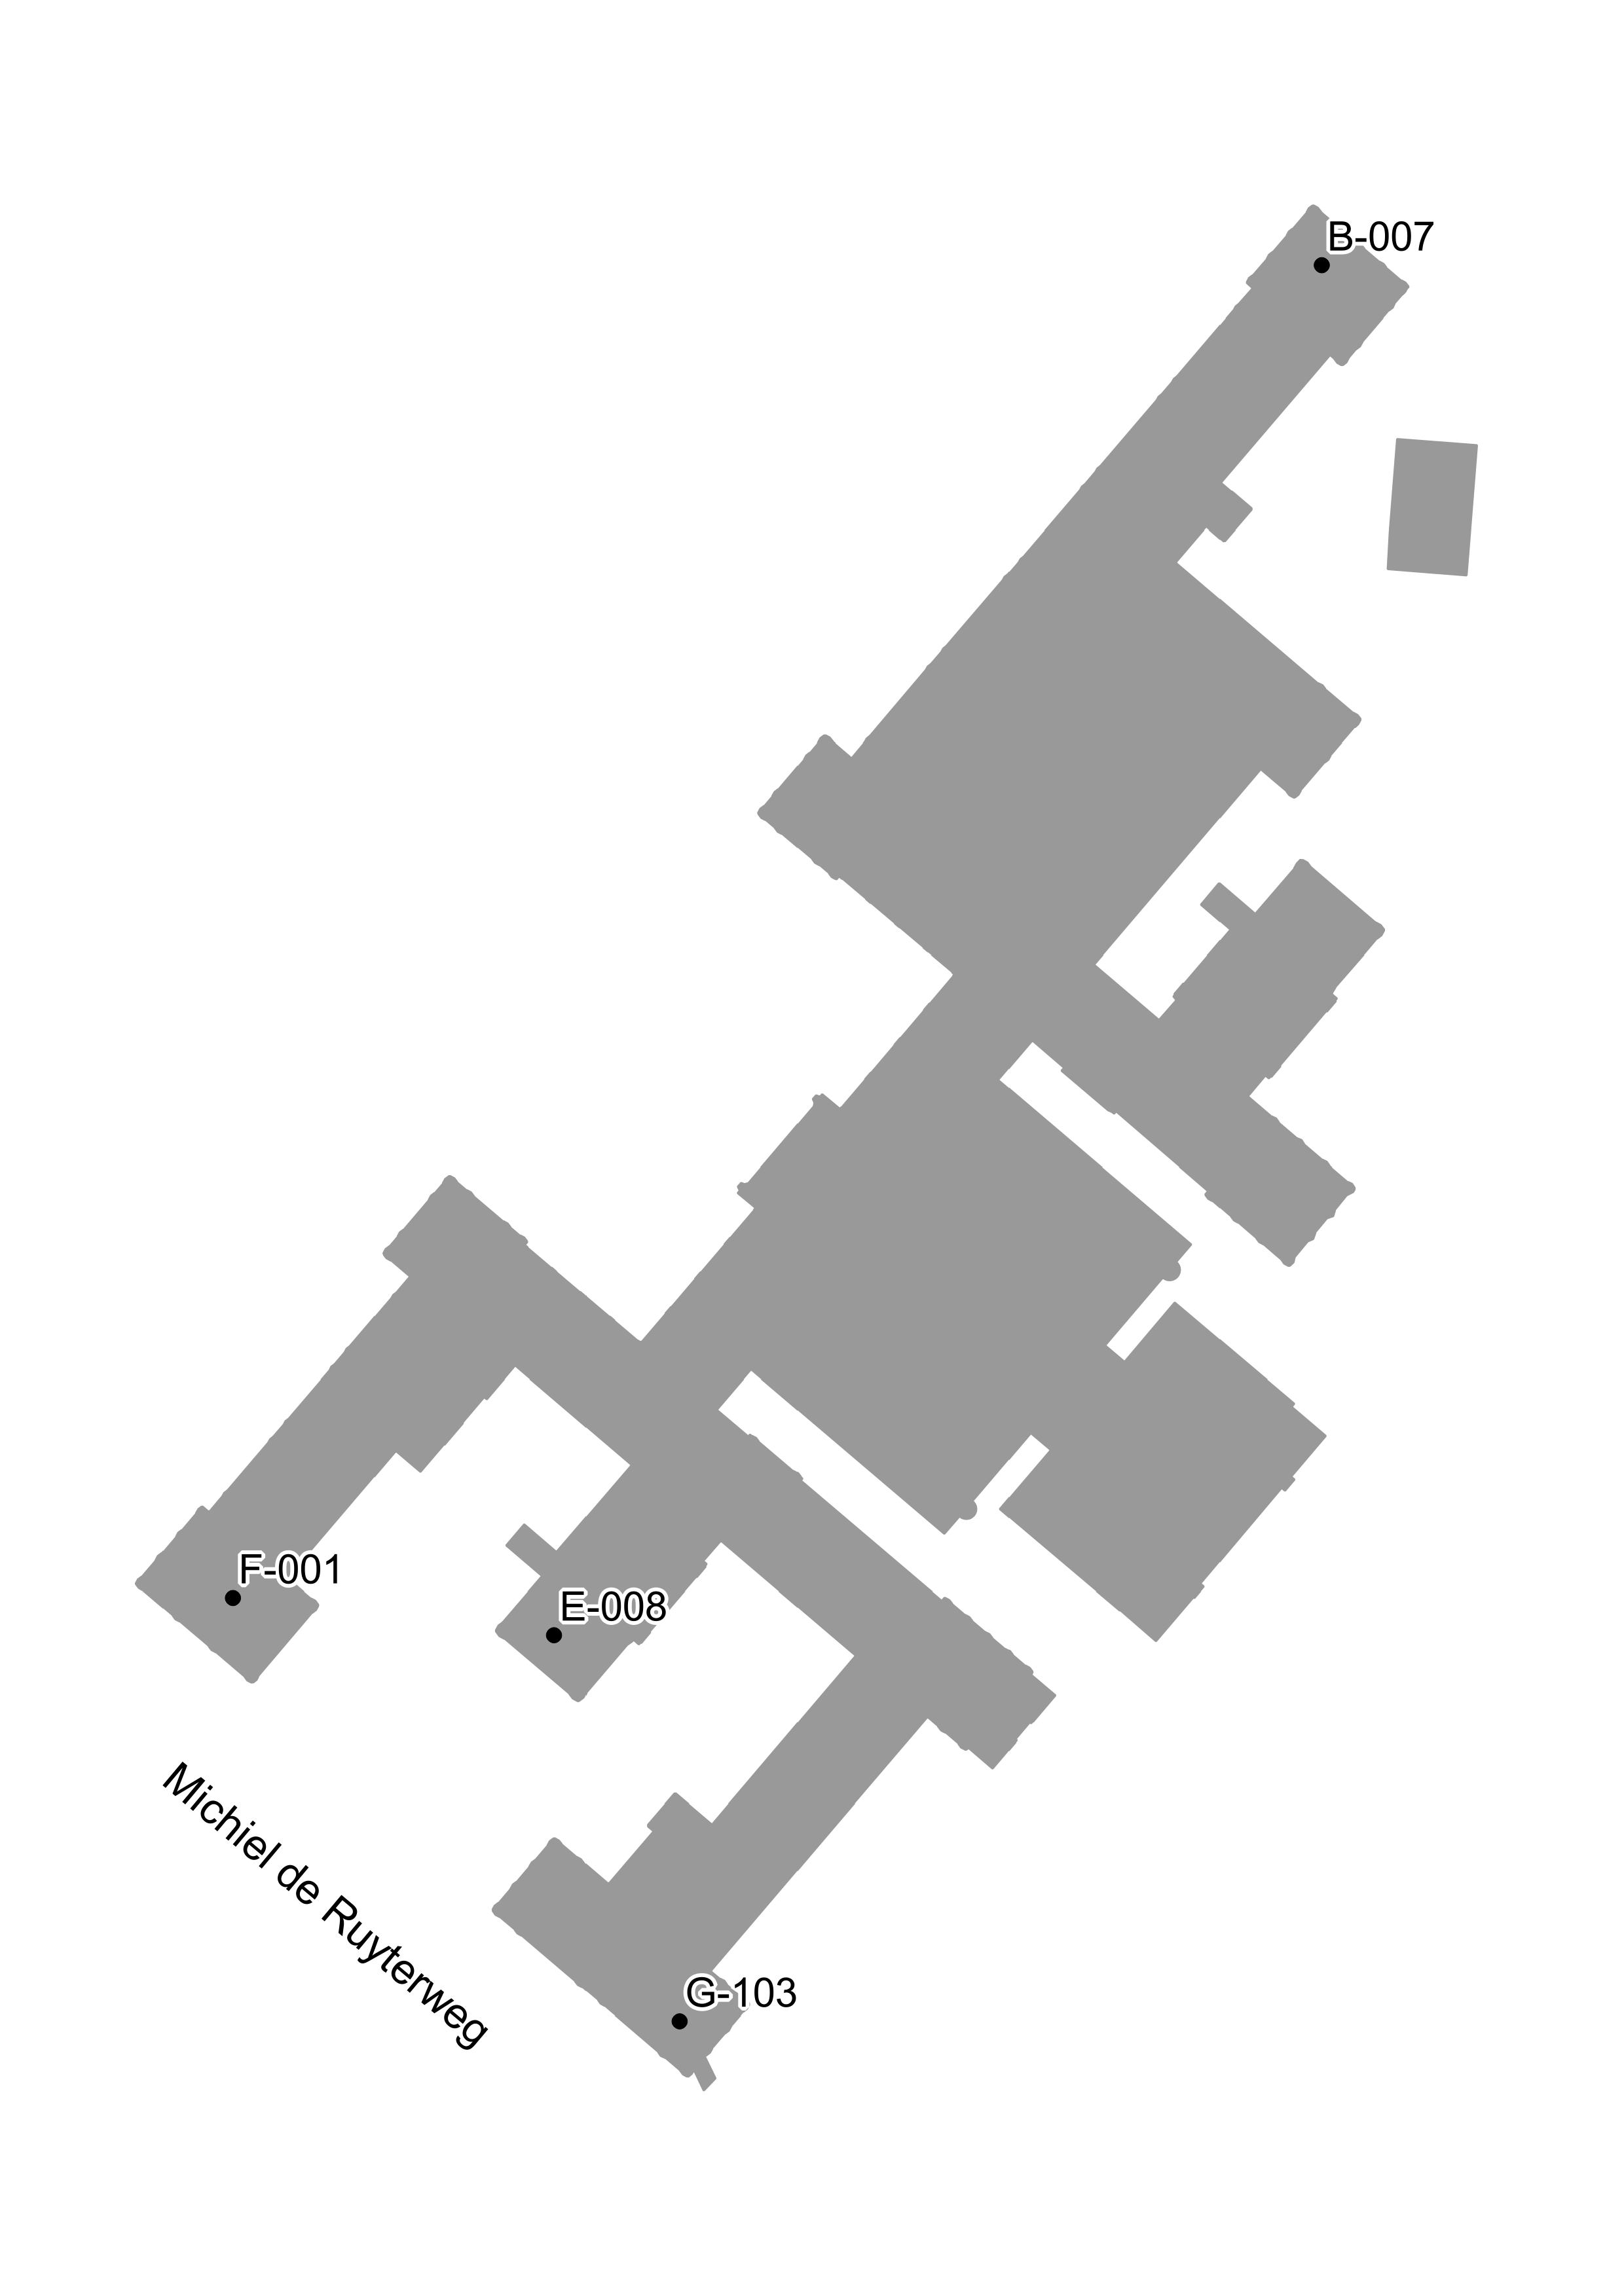
\includegraphics[scale=0.3]{bk_aplocs1.png}
	\captionsetup{justification=centering}
	\caption{The location of the most frequently used APs that are used to record the first and/or last connection of a device in the Faculty of Architecture}
	\label{firstapproach_map}
\end{figure}
\subsection{Second approach: excluding passing by events}
Table x shows the individual states as a result of the pre-processing (see chapter pre-processing). The records represent the states for each mac, including the first and last recorded AP (ap\_start, ap\_end). \\\\
\begin{table}[H]
	\centering
	\captionsetup{justification=centering}
	\caption{Individual states as a result of the pre-processing}
	\label{individualstates}
	\begin{tabular}{@{}llllll@{}}
		\toprule
		\textbf{mac} & \textbf{building} & \textbf{ts}     & \textbf{te}     & \textbf{ap\_start} & \textbf{ap\_end} \\ \midrule
		000c+YfkIi.. & 0                 & 30-3-2016 23:34 & 6-4-2016 22:39  & NULL               & NULL             \\
		000c+YfkIi.. & 21                & 6-4-2016 22:39  & 6-4-2016 23:30  & A-21-0-005         & A-21-0-045       \\
		000c+YfkIi.. & 0                 & 6-4-2016 23:40  & 10-4-2016 19:53 & NULL               & NULL             \\
		000c+YfkIi.. & 0                 & 10-4-2016 20:03 & 10-4-2016 21:13 & NULL               & NULL             \\
		000c+YfkIi.. & 21                & 10-4-2016 21:13 & 10-4-2016 21:34 & A-21-0-046         & A-21-0-046       \\
		000c+YfkIi.. & 21                & 10-4-2016 22:04 & 10-4-2016 22:19 & A-21-0-045         & A-21-0-046       \\
		000c+YfkIi.. & 0                 & 10-4-2016 22:19 & 10-4-2016 23:14 & NULL               & NULL             \\
		000c+YfkIi.. & 0                 & 10-4-2016 23:24 & 11-4-2016 12:27 & NULL               & NULL             \\
		000c+YfkIi.. & 21                & 11-4-2016 12:27 & 11-4-2016 13:25 & A-21-0-043         & A-21-0-043       \\
		000c+YfkIi.. & 20                & 11-4-2016 13:25 & 11-4-2016 13:56 & A-20-0-008         & A-20-0-045       \\ \bottomrule
	\end{tabular}
\end{table}
The table also includes ’world’ (in \autoref{individualstates} represented by NULL) which implies the device is not located on the campus. A simple SQL query is used for plotting the most frequently used first and last recorded APs in a stay (\autoref{secondapproach_graph})\\\\
\begin{figure}[H]
	\centering
	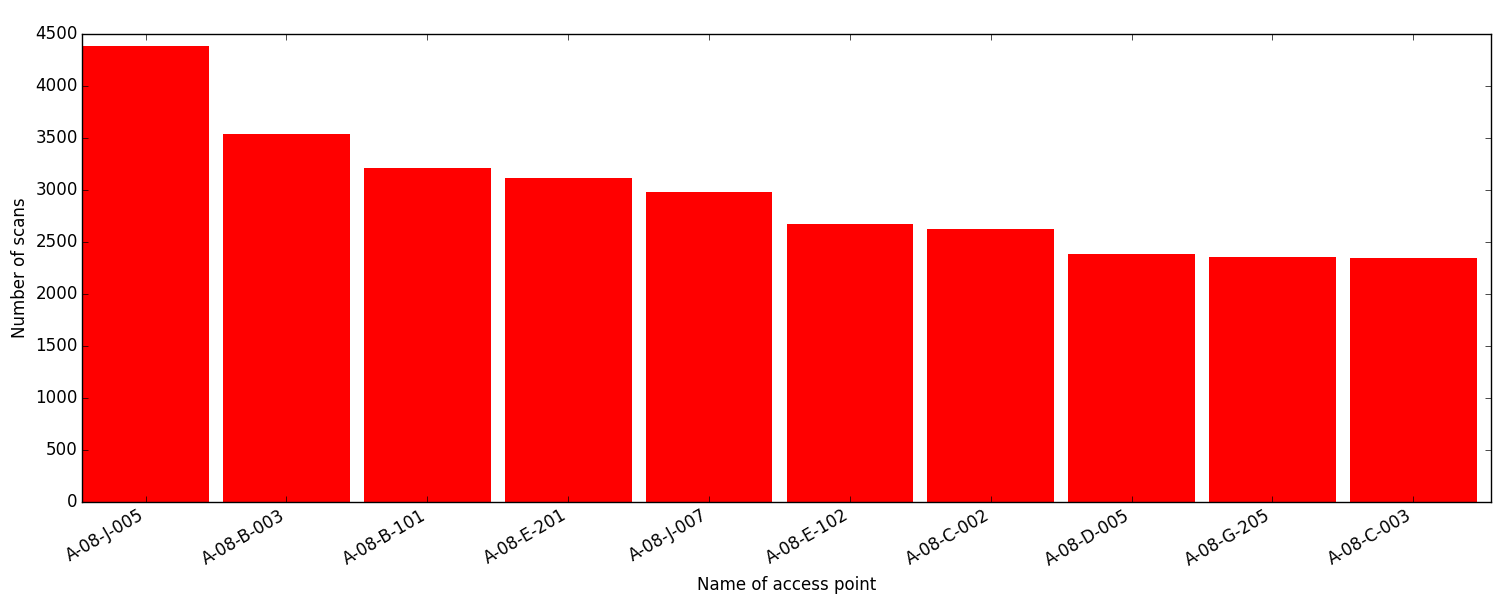
\includegraphics[scale=0.2]{entrances_secondapproach_1.png}
	\captionsetup{justification=centering}
	\caption{Most frequently recorded APs in a movement to the Faculty of Architecture}
	\label{secondapproach_graph}
\end{figure}
\begin{figure}[H]
	\centering
	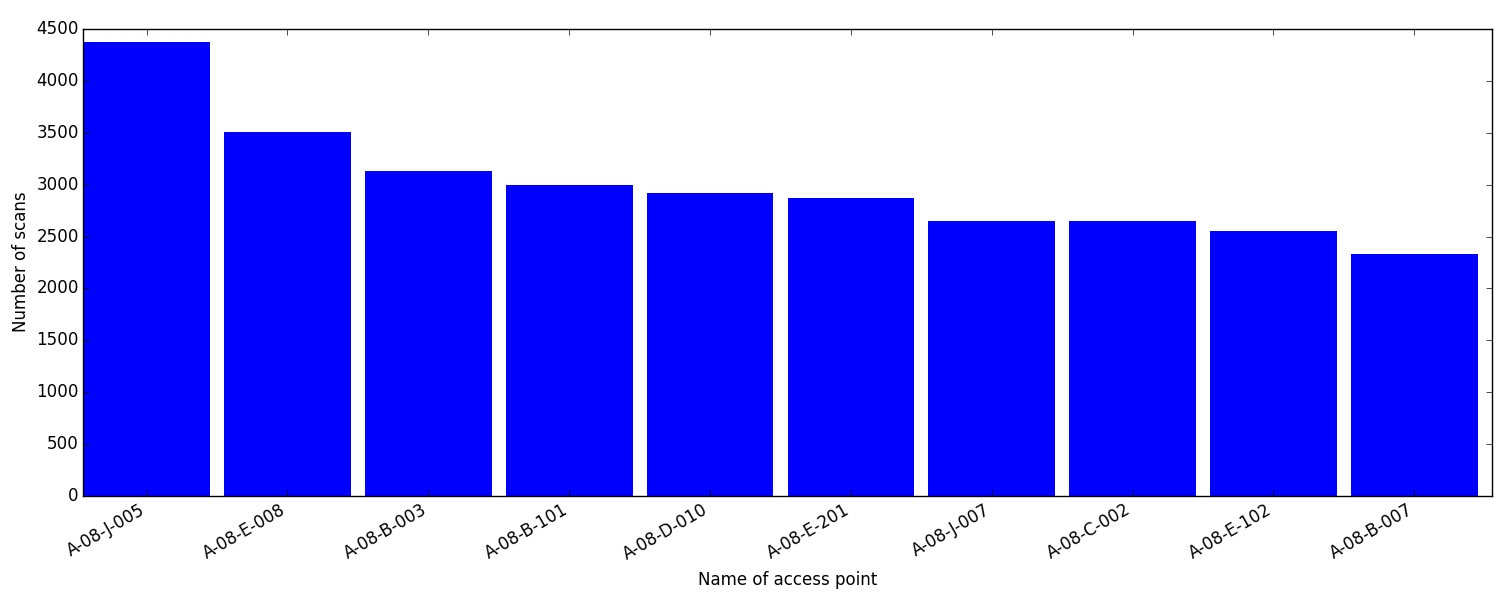
\includegraphics[scale=0.2]{entrances_secondapproach_2.png}
	\captionsetup{justification=centering}
	\caption{Most frequently recorded APs in a movement from the Faculty of Architecture}
	\label{secondapproach_graph}
\end{figure}
The most frequently used access point, A-08-J-005, is located high up in the modelling hall and thus not near an entrance (see \autoref{secondapproach_map}). Although this location is different than expected there might be a reason for it. The access point is placed in an open space in which no objects could seriously block the Wi-Fi signal.
\begin{figure}[H]
	\centering
	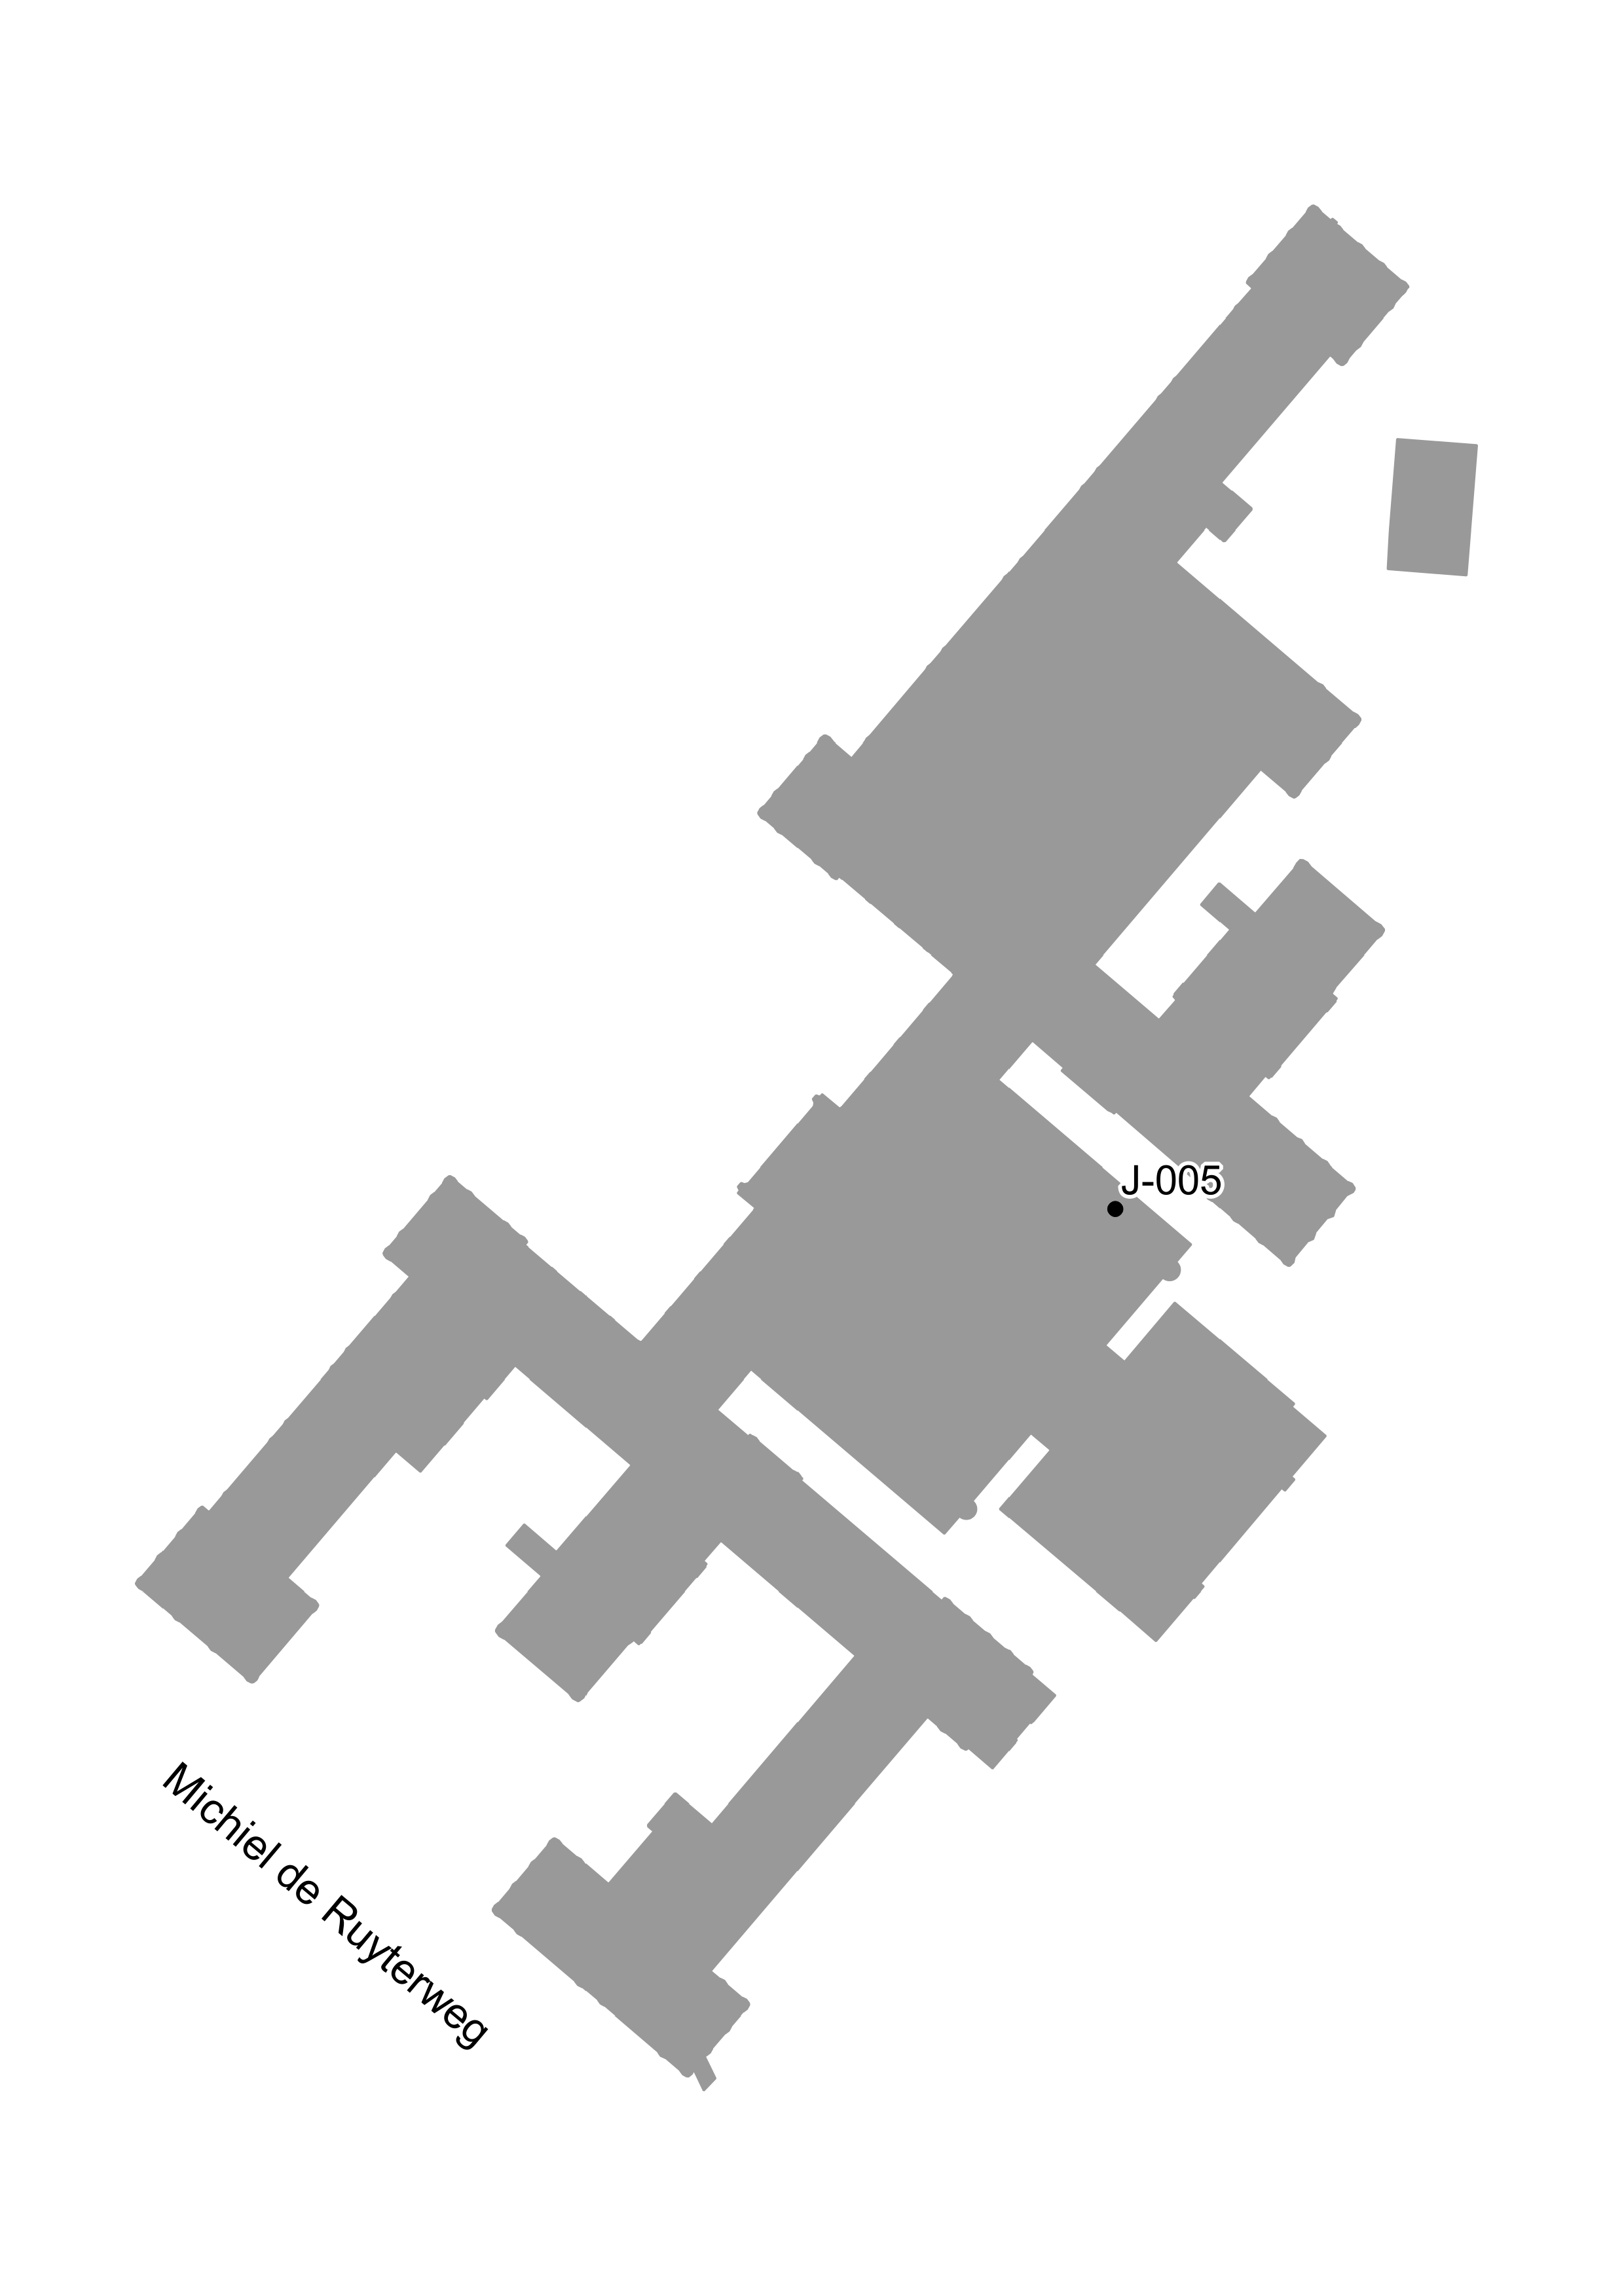
\includegraphics[scale=0.3]{bk_aplocs2.png}
	\captionsetup{justification=centering}
	\caption{The location of the most frequently used APs that are used to record the first and/or last connection of a device in the Faculty of Architecture}
	\label{secondapproach_map}
\end{figure}
In order to know with what APs a device connects when entering a building, some experiments are conducted. By looking at the MAC address of the access point the device is connects with, it would be possible to identify the location of that AP. This experiment is conducted for entering the Faculty of Architecture via the East, West and main entrance. \autoref{entrance_experiment_results} shows the results of the experiment.\\\\
\begin{table}[H]
	\centering
	\captionsetup{justification=centering}
	\caption{The AP a device connects with when entering the Faculty of Architecture}
	\label{entrance_experiment_results}
	\begin{tabular}{@{}llll@{}}
		\toprule
		\textbf{entrance} & \textbf{MAC address} & \textbf{apname} & \textbf{maploc}    \\ \midrule
		east entrance     & 00-15-C7-80-9A-60    & not found       & not found          \\
		west entrance     & 00-22-90-5E-66-F0    & A-09-E-102      & 1st floor West MSc \\
		main entrance     & 00-22-90-38-7F-D0    & not found       & not found          \\ \bottomrule
	\end{tabular}
\end{table}
The AP a device connects with when entering the building via the West entrance, E-102', can also be found in \autoref{secondapproach_graph}. Though it does not stand out compared to other APs. The MAC addresses of the APs the device connects with when entering the building via the East or Main entrance are not found, meaning the APs are not located on the map or listed in the table of APs. This implies it is not possible to relate the results to the data. 
\subsection{Recommendation}
The results and conducted experiments has shown it is not possible to clearly find what, when and how frequent entrances of the Faculty of Architecture are used. The first and most important reason for that, is the time interval of approximately 5 minutes in which the system is recording. A person could be anywhere in the building at the moment of recording. A smaller time interval between the moments of recording would help in finding answers to the questions regarding the use of the entrances. Also, the existing layout of APs in the Faculty of Architecture is currently not designed for any other purpose than allowing a Wi-Fi compliant device to connect with the wireless eduroam network. Locating APs near the entrances of a building might help. Moreover, the fact the Faculty of Architecture has multiple entrances, in combination with the large time interval of recording, is what makes identification of the entrances difficult. 
\section{Association rules} 
% Balazs

\section{Distinguishing user groups}
% Simon
% People moving in groups

\section{Occupancy}
% Matthijs

\section{AP system}
% Matthijs
% Scan time, also outdoors maybe?
The setup of the system that logs the devices connected to access points is directly connected to the accuracy of the processed data. Currently, the APs register every device that is connected to it and the logging system receives all connected devices approximately every five minutes. Additionally, all access points are located indoors, logging every device carried by people using that building. These two aspects of the AP system limit the accuracy of the processed data and thus the movement patterns that can be derived. \\\\
Because the system logs every connected devices once every five minutes, a device will only be registered if the devices is connected for at least five minutes (not really true). This will result in discrepancies in the processed data. Devices and thus people walking by an AP will probably not be registered, for they are not connected to that AP for at least five minutes. This is unfortunate, because a person can travel a rather long distance in five minutes, e.g. making it hard to track people indoors. If the system would be logging every device all the time, irrespective of the time the device is connected, the tracking data would contain every AP that a device would connect to and thus provide much more accurate tracking data. Understandably, logging every user every second would result in huge amounts of data, which would most definitely result in performance issues.\\\\
Secondly, because all scanners are located inside buildings, there is little to no information on people when they move from one building to another. Surely something can be told from the time it takes a device from the last scan in one building, to the first scan in the second building. But for outdoor tracking purposes, this system is limited. From some experiments that were conducted on the TU Delft Campus it can be concluded that a device located outdoors near a building can be detected by APs inside the building, but this depends on the antenna in the devices and the exact location of the device in respect to the AP. If more detailed information about movement outdoors is desired, it would be wise to also include outdoor APs in the system.\\\\
To improve further research, it is recommended to take the system of APs into account before actually conducting the research. If outdoor movement tracking is desired, outdoor APs are required. And if tracking indoors is one of the goals, the frequency of logging should be set to an interval that is in the order of magnitude of 10 seconds to one minute, taking data size in consideration.

\section{Data reasoning}
% Simon
During this project a lot of data is handled. With all the data available and the processing to derive movement patterns one could ask: 'How reliable is the data?' and 'How accurately can we derive these movement patterns?'. Determining the working of the system of APs as described in \autoref{apsystem}, was a great step towards a reliable outcome. Knowing how the system works helped improve the processing steps that were taken, because the systems flaws could be taken into account and avoided. Additionally, when the first movement patterns were derived, common knowledge and knowledge about the TU Delft campus and its layout helped in validating these patterns.\\\\
Because the working of the system of APs is known, the dataset can be improved by filtering out people that are only registered for less than five minutes at one AP, indicating that they only were only passing by. This means that the states derived from the data are actually stay places of an individual. Another perspective could be that exactly those people that are only passing by are valuable for the dataset. When an individual is registered at four consecutive APs and each scan was less than five minutes, it can be concluded that this person is moving between those four APs. However, the current set-up of the AP system is not suitable enough to use only devices that have a session duration of less than five minutes. This would only work when the frequency of loggin is increased.\\\\
Moreover, the knowledge acquired from previous courses in the Geomatics programme and common knowledge about buildings and the TU Delft campus can be used to validate certain outcomes of the data processing. For example, it would seems very illogical that an individual could travel from Architecture to Aerospace Engineering and then to Industrial Design in five minutes. Such requirements could improve the final outcomes. This kind of reasoning became even more useful when zooming in to spatial level buildingpart. Using the knowledge of the building layout of Architecture, it could be concluded that moving from one floor to another is impossible without using one of the staircases. Such a conclusion could then be included in the processing, e.g. validating only movement between floors if one of the staircases is used. \\\\
For future research, it is desirable to use a higher frequency for logging the connected devices. This will ensure that a device is always registered and that its movement can be easily identified. Furthermore, %<-- Simon insert something about data reasoning and trajectories here -->%

\section{Visual exploration}
% Ethan/Matthijs
% What did and didnt work
